\Needspace{8\baselineskip}\originalchapter{习题课: 场方程、旋量与振幅}
本章收录Recitation 6--11及12题2。先用ABC标量模型把顶点、传播子与相空间分开，再把同样步骤应用于Dirac流、QED与QCD。所有质量和动量采用$c=1$；若宽度以能量给出，寿命为$\hbar/\Gamma$，不能把能量宽度与每秒衰变率混写。原件图中的物种、动量和颜色标签在新绘图与题干中保留。
\originalsection{ABC模型的低阶过程}
\begin{exercise}\label{ex:rec-6-1}
Recitation 6题1。求课堂ABC toy theory中粒子$A$的寿命。为使题面自足：三个不同实标量场的相互作用为$\Lag_{\rm int}=-gABC$，顶点$-\ii g$，各传播子$\ii/(q^2-m^2+\ii0)$，假设$m_A>m_B+m_C$。
\end{exercise}
\begin{solution}
官方树图与相空间结果重编。$A\to B+C$只有一个顶点，$|\mathcal M|^2=g^2$。对$A$静止系的两体相空间积分，
\begin{equation}
 p_* =\frac{\sqrt{[m_A^2-(m_B+m_C)^2][m_A^2-(m_B-m_C)^2]}}{2m_A},
 \qquad\Gamma_E=\frac{g^2p_*}{8\pi m_A^2},\qquad\tau=\frac{\hbar}{\Gamma_E}.
\end{equation}
$B,C$是不同粒子，没有同粒子$1/2!$。若阈值未达到，此实两体道的宽度为零，不能继续使用虚数$p_*$作寿命。求$p_*$的完整运动学证明见习题\ref{ex:8701-2-2}，此题还要求把该结果接到衰变率，故并非同一题的重复计数。
\begin{center}\begin{tikzpicture}[scale=.85]
\draw(-1.5,0)--(0,0)node[midway,above]{$A$};\draw(0,0)--(1.5,.8)node[right]{$B$};\draw(0,0)--(1.5,-.8)node[right]{$C$};\fill(0,0)circle(2pt);
\end{tikzpicture}\end{center}
\end{solution}
\begin{exercise}\label{ex:rec-6-2}
Recitation 6题2。求$A+A\to B+B$微分截面。使用前题ABC规则；原题未指定质量，先给一般树级式，再按官方解答的特例$m_A=m_B=m,m_C=0$化简，质心每束总能量$E$、动量大小$p$、散射角$\theta$。
\end{exercise}
\begin{solution}
官方两图重绘与结果复算。两个末态$B$可交换，有$t$、$u$两图，取振幅的同一整体符号约定，
\begin{equation}
 \mathcal M=g^2\left[\frac1{t-m_C^2}+\frac1{u-m_C^2}\right],\quad
 \frac{\dd\sigma}{\dd\Omega}=\frac1{2!}\frac1{64\pi^2s}\frac{p_B}{p_A}|\mathcal M|^2.
\end{equation}
这里按完整立体角积分，$1/2!$消除同一末态配置被重复计数；若只积不重叠半球则去掉该因子。
特例中$s=4E^2,p^2=E^2-m^2$，$t=-2p^2(1-\cos\theta)$、$u=-2p^2(1+\cos\theta)$，故
\begin{equation}
 \mathcal M=-\frac{g^2}{p^2\sin^2\theta},\qquad
 \frac{\dd\sigma}{\dd\Omega}=\frac{g^4}{512\pi^2E^2p^4\sin^4\theta}.
\end{equation}
恢复自然单位面积需乘$(\hbar c)^2$。两端发散来自无质量$C$的长程交换，不能声称有有限总截面；有限角接受度或屏蔽尺度才可截断。既有习题\ref{ex:8701-2-4}取$m_B=m_C=0$、入射$A$有质量，运动学不同，不能以其截面替代本题。
\begin{center}\begin{tikzpicture}[scale=.65]
\foreach\x/\cross/\tag in{0/0/t,6/1/u}{
\fill(\x,1)circle(2pt);\fill(\x,-1)circle(2pt);
\draw(\x-1.4,1.6)--(\x,1)node[midway,above]{$A_1$};\draw(\x-1.4,-1.6)--(\x,-1)node[midway,below]{$A_2$};
\draw[dashed](\x,1)--(\x,-1)node[midway,right]{$C$};
\draw(\x,1)--(\x+1.4,1.6)node[right]{$B_{\ifnum\cross=0 3\else4\fi}$};
\draw(\x,-1)--(\x+1.4,-1.6)node[right]{$B_{\ifnum\cross=0 4\else3\fi}$};
\node at(\x,-2.2){$\tag$道};}
\end{tikzpicture}\end{center}
\end{solution}
\begin{exercise}\label{ex:rec-7-1}
Recitation 7题1。(a)$A\to B+B$在ABC理论中允许吗？(b)若图有$n_A,n_B,n_C$条各类外腿，建立允许反应的简单判据；(c)假设$A$足够重，除$A\to B+C$外最可能的衰变模式是什么？画各衰变图。
\end{exercise}
\begin{solution}
官方外腿计数与四体图重编，动力学条件补全。若图有$V$个ABC顶点、$I_s$条物种$s$内部线，则每种场的端点数均为$V$，所以
\begin{equation}n_s=V-2I_s\quad(s=A,B,C).\end{equation}
三个$n_s$必须同为奇数或同为偶数。$A\to BB$给$(1,2,0)$，因而禁戒。反过来同奇偶可配对相应端点构造形式图；需允许足够多顶点，不能把不相连的最少顶点图当作连通散射图。这项端点判据也由同时改变任意两场符号的$Z_2$对称性解释；它不替代质量阈值、连通性和具体振幅计算。

只有末态$B,C$的较高道中，三个末粒子无法使$n_B,n_C$均奇；四体允许$A\to3B+C$与$A\to B+3C$，树图最少三个顶点，振幅阶$g^3$、宽度阶$g^6$，并各有三个相同粒子的相空间因子。含末态$A$的低阶道会因母粒子质量不足关闭。以下各给一张代表图，同类末腿置换也须计入；“最可能的下一类”指耦合阶数，两个四体道谁更大仍取决于质量和相空间。
\begin{center}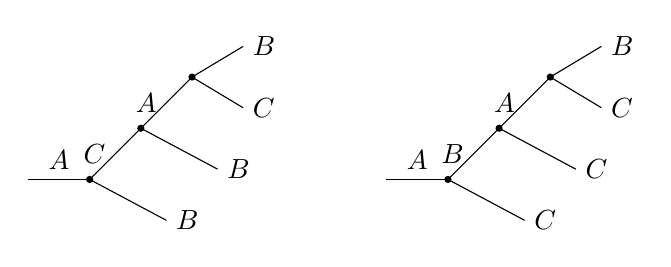
\begin{tikzpicture}[scale=.65]
\foreach\x/\first/\outa/\outb/\last in{0/C/B/B/C,7/B/C/C/B}{
\draw(\x-1.2,0)--(\x,0)node[midway,above]{$A$};
\draw(\x,0)--(\x+1,1)node[midway,left]{$\first$};\draw(\x,0)--(\x+1.5,-.8)node[right]{$\outa$};
\draw(\x+1,1)--(\x+2,2)node[midway,left]{$A$};\draw(\x+1,1)--(\x+2.5,.2)node[right]{$\outb$};
\draw(\x+2,2)--(\x+3,2.6)node[right]{$B$};\draw(\x+2,2)--(\x+3,1.4)node[right]{$C$};
\foreach\a/\b in{0/0,1/1,2/2}\fill(\x+\a,\b)circle(2pt);}
\end{tikzpicture}\end{center}
\end{solution}
\originalsection{Dirac代数、共变电磁场与伴随旋量}
\begin{exercise}\label{ex:rec-8-1}
Recitation 8题1。分别考虑$\mu=\nu=0$、$\mu=\nu\ne0$及$\mu\ne\nu$，证明$\gamma^\mu\gamma^\nu+\gamma^\nu\gamma^\mu=2g^{\mu\nu}I_4$。
\end{exercise}
\begin{solution}
官方提示扩为完整分块检查。采用$g=\diag(1,-1,-1,-1)$及
\begin{equation}
\gamma^0=\diag(I_2,-I_2),\qquad
\gamma^i=\begin{pmatrix}0&\sigma_i\\-\sigma_i&0\end{pmatrix}.
\end{equation}
$\sigma_i\sigma_j+\sigma_j\sigma_i=2\delta_{ij}I_2$给$(\gamma^0)^2=I_4$、$(\gamma^i)^2=-I_4$；当$\mu=\nu$时即得对应$\pm2I_4$。
异指标中$\gamma^0\gamma^i$与$\gamma^i\gamma^0$的非对角块相反；两个不同空间指标给$-\{\sigma_i,\sigma_j\}$的对角块，等于零。三类穷尽全部指标。
\end{solution}
\begin{exercise}\label{ex:rec-8-2}
Recitation 8题2。质心系中$e^+e^-\to\gamma^*\to e^+e^-$，中间光子能量为$2E$。分别以(a)负能粒子向时间反方向传播，(b)正能反粒子向时间正方向传播的解释，讨论能量和电荷守恒。
\end{exercise}
\begin{solution}
官方Feynman--Stueckelberg解释重编。质心系$q=(2E,\mathbf0)$，$q^2=4E^2>0$，所以中间是虚光子，不是可静止的实光子。
(a)顺着电子费米子线在第一顶点看：$+E=(-E)+2E$，电荷沿整条电子线均为$-e$；负能分支的时序相反。第二顶点为$-E+2E=+E$。
(b)把负能反向段重新解释为正能正电子入/出射，第一顶点$E+E=2E$且$-e+e=0$，第二顶点反之。两种图的同一内部线计数与守恒量相同；重解释不能当作可观测粒子违反时间因果的运动。
\begin{center}\begin{tikzpicture}[scale=.75]
\draw[fermion](-1.5,-1)--(0,0);\draw[fermion](0,0)--(-1.5,1);
\draw[photon](0,0)--(2,0)node[midway,above]{$\gamma^*,\ 2E$};
\draw[fermion](2,0)--(3.5,1);\draw[fermion](3.5,-1)--(2,0);
\node at(-1.8,-1.3){$e^-,+E$};\node at(-1.8,1.3){$e^+,+E$};
\node at(3.8,1.3){$e^-,+E$};\node at(3.8,-1.3){$e^+,+E$};
\draw[->](-3,-1)--(-3,1)node[above]{时间};
\end{tikzpicture}\end{center}
费米子线箭头表示电荷流向，正电子的箭头与它的正向时间传播方向相反。
\end{solution}
\begin{exercise}\label{ex:rec-9-1}
Recitation 9题1。从$\partial_\mu F^{\mu\nu}=4\pi J^\nu/c$推导
$\nabla\cdot\mathbf E=4\pi\rho$及$\nabla\times\mathbf B-c^{-1}\partial_t\mathbf E=4\pi\mathbf J/c$。本题沿源件使用Gaussian单位，$x^0=ct,J^\mu=(c\rho,\mathbf J)$。
\end{exercise}
\begin{solution}
官方逐指标解重编。为与所给方程同号，取$F^{i0}=E_i,F^{0i}=-E_i,F^{ij}=-\epsilon_{ijk}B_k$。
$\nu=0$时$\partial_iF^{i0}=\partial_iE_i=4\pi\rho$。
$\nu=1$时
\begin{equation}
 \partial_\mu F^{\mu1}=-\frac1c\partial_tE_x+\partial_yB_z-\partial_zB_y
 =\frac{4\pi}{c}J_x.
\end{equation}
$\nu=2,3$给另外两分量，合成所求Ampere--Maxwell式。若教材定义$F$为本式的相反数，场方程源项也要相应改号；不能混取不同惯例。SI单位须整体换成$\epsilon_0,\mu_0$，而非只替换$4\pi$。
\end{solution}
\begin{exercise}\label{ex:rec-9-2}
Recitation 9题2。证明由$F^{\mu\nu}$反对称性得到的$\partial_\mu J^\mu=0$保证电荷守恒。
\end{exercise}
\begin{solution}
官方思路重编。光滑场导数可交换，$\partial_\nu\partial_\mu$对指标对称，与$F^{\mu\nu}$收缩为零，于是$\partial_\nu J^\nu=0$。用上一题坐标即$\partial_t\rho+\nabla\cdot\mathbf J=0$。固定区域$V$积分并用Gauss定理，
\begin{equation}\frac{\dd}{\dd t}\int_V\rho\dd^3x=-\oint_{\partial V}\mathbf J\cdot\mathbf n\dd S.\end{equation}
局域守恒指区域电荷变化正是流出通量；只有封闭无通量边界或全空间无穷远通量消失时，区域总电荷才恒定。
\end{solution}
\begin{exercise}\label{ex:rec-10-1}
Recitation 10题1。证明伴随旋量满足$\bar u(\gamma^\mu p_\mu-m)=0$、$\bar v(\gamma^\mu p_\mu+m)=0$。
\end{exercise}
\begin{solution}
官方分块共轭证明重编。原方程为$(\slashed p-m)u=0$、$(\slashed p+m)v=0$。Pauli矩阵Hermitian，故$(\gamma^0)^\dagger=\gamma^0$、$(\gamma^i)^\dagger=-\gamma^i$，统一写成$(\gamma^\mu)^\dagger\gamma^0=\gamma^0\gamma^\mu$。取Hermitian共轭、右乘$\gamma^0$，得$u^\dagger\gamma^0(\slashed p-m)=0$及$v^\dagger\gamma^0(\slashed p+m)=0$。定义$\bar u=u^\dagger\gamma^0,\bar v=v^\dagger\gamma^0$便得所求；$p_\mu$为实在壳四动量。
\end{solution}
\begin{exercise}\label{ex:rec-10-2}
Recitation 10题2。证明协变归一化$\bar u u=-\bar v v=2m$。注意原PDF是此标量乘积；文本提取中乘法次序曾倒置，不能写成矩阵外积$u\bar u$。
\end{exercise}
\begin{solution}
官方分块计算重编。对归一化二旋量$\chi^\dagger\chi=\eta^\dagger\eta=1$，
\begin{equation}
 u=\sqrt{E+m}\begin{pmatrix}\chi\\\frac{\boldsymbol\sigma\cdot\mathbf p}{E+m}\chi\end{pmatrix},\quad
 v=\sqrt{E+m}\begin{pmatrix}\frac{\boldsymbol\sigma\cdot\mathbf p}{E+m}\eta\\\eta\end{pmatrix}.
\end{equation}
$\gamma^0$给上块减下块；利用$(\boldsymbol\sigma\cdot\mathbf p)^2=p^2I_2$与$E^2-p^2=m^2$，
$\bar u u=(E+m)-p^2/(E+m)=2m$、$\bar v v=p^2/(E+m)-(E+m)=-2m$。
同时$u^\dagger u=v^\dagger v=2E$。无质量极限的协变标量归一化趋零，却不表示正定密度归一化为零。
\end{solution}
\originalsection{颜色、真空极化与可观测截面}
\begin{exercise}\label{ex:rec-11-1}
Recitation 11题1。定义$R=\sigma(e^+e^-\to\mathrm{hadrons})/\sigma(e^+e^-\to\mu^+\mu^-)$。(a)此比值能告诉我们什么？(b)若分母改为电子--正电子弹性末态，结果如何改变？求相应关系。
\end{exercise}
\begin{solution}
官方要点扩为可计算式。远离共振、忽略质量且取单光子最低阶，$\sigma_{\mu\mu}=4\pi\alpha^2/(3s)$；每种夸克的电荷平方与颜色多重性给
$R=N_c\sum_{\rm open}Q_q^2$。依次开放$u,d,s$时为2，再开$c$为$10/3$，再开$b$为$11/3$。测阶梯可检验电荷、可达味与$N_c=3$；阈值、强子共振及QCD修正使真实曲线不是理想阶梯，连续区第一修正约$1+\alpha_s/\pi$。

电子末态除$s$道外还有$t$道Bhabha图及干涉，其前向极点使全角总截面在无质量近似下发散。给定角接受区$\mathcal A$才可定义
$R_e(\mathcal A)=\sigma_h(\mathcal A)/\sigma_{ee}(\mathcal A)$；它不再让运动学因子抵消，原题没有角切条件，因而没有唯一数值。不能把分母简单改一个轻子标签。
\end{solution}
\begin{exercise}\label{ex:rec-11-2}
Recitation 11题2。画含夸克、胶子的真空极化图，讨论QED与QCD真空极化的差异。
\end{exercise}
\begin{solution}
官方答案仅指向Lecture5.5，以下据该课程主题补完整说明。QED光子可接带电费米子闭环，夸克环须求电荷平方和并乘颜色数；光子不带电，没有基本光子自耦合环。QCD的外胶子既可接夸克环，也有胶子自耦合环、四胶子项，协变规范还需ghost环。ghost不是可观测外态，而是保持规范量子计算一致性的内部贡献。
\begin{center}\begin{tikzpicture}[scale=.7]
\foreach\x/\mode/\lab in{0/0/夸克环,4/1/胶子环,8/2/ghost环}{
\draw[photon](\x-1.4,0)--(\x-.7,0);\draw[photon](\x+.7,0)--(\x+1.4,0);
\ifnum\mode=0\draw[fermion](\x+.7,0)arc(0:180:.7);\draw[fermion](\x-.7,0)arc(180:360:.7);
\else\ifnum\mode=1\draw[photon](\x+.7,0)arc(0:180:.7);\draw[photon](\x-.7,0)arc(180:360:.7);
\else\draw[dashed,->](\x+.7,0)arc(0:180:.7);\draw[dashed,->](\x-.7,0)arc(180:360:.7);\fi\fi
\node at(\x,-1.3){\lab};}
\end{tikzpicture}\end{center}
环图应按横向张量$\Pi_{\mu\nu}=(q_\mu q_\nu-q^2g_{\mu\nu})\Pi(q^2)$组合。QED费米子屏蔽使$\alpha(Q)$随尺度增长；QCD胶子项的反屏蔽给
\begin{equation}\frac{\dd\alpha_s}{\dd\ln Q}=-\frac{\beta_0}{2\pi}\alpha_s^2,\qquad \beta_0=11-\frac23N_f,\end{equation}
所以通常可达$N_f$下高能耦合变小。上图是三类环拓扑示意，另有四胶子顶点形成的圈图；每类的组合、反项与系数均须按所选规范计算，不能仅凭图数读出$\beta_0$。
\end{solution}
\begin{exercise}\label{ex:rec-12-2}
Recitation 12题2。求原图$s$道单胶子$q(p_1,c_1)+\bar q(p_2,c_2)\to q(p_3,c_3)+\bar q(p_4,c_4)$的振幅与颜色因子$f$；在色单态配置下算$f$并解释。内线$q=p_1+p_2=p_3+p_4$，顶点$-\ii g_s\gamma^\mu T^a$、$T^a=\lambda^a/2$。
\begin{center}\begin{tikzpicture}[scale=.8]
\draw[fermion](-1.6,-1)--(0,0);\draw[fermion](0,0)--(-1.6,1);
\draw[photon](0,0)--(2,0)node[midway,above]{$g^a,q$};
\draw[fermion](2,0)--(3.6,1);\draw[fermion](3.6,-1)--(2,0);
\node[left]at(-1.6,-1){$p_1,c_1$};\node[left]at(-1.6,1){$p_2,c_2$};
\node[right]at(3.6,1){$p_3,c_3$};\node[right]at(3.6,-1){$p_4,c_4$};
\end{tikzpicture}\end{center}
\end{exercise}
\begin{solution}
官方单态零因子重编。忽略整体振幅号，
\begin{equation}
 \mathcal M=\frac{g_s^2}{q^2}
 [\bar v_2\gamma^\mu u_1][\bar u_3\gamma_\mu v_4]\,f,\qquad
 f=\sum_a(c_2^\dagger T^ac_1)(c_3^\dagger T^ac_4).
\end{equation}
对归一化单态$\ket{\mathbf1}=\sum_i\ket{i\bar i}/\sqrt3$，单胶子耦合为$\sum_i(T^a)_{ii}/\sqrt3=\Tr T^a/\sqrt3=0$，所以此$s$道图的$f=0$。这是单态不能通过一个八重态胶子转变的选择定则；不意味着色单态系统所有QCD振幅都为零。特别不能把另一$t$道的吸引因子$-4/3$代入此原图。
\end{solution}
